\documentclass[12pt]{article}

\usepackage{amssymb,amsmath,amsfonts,eurosym,geometry,ulem,graphicx,caption,color,setspace,sectsty,comment,footmisc,caption,natbib,pdflscape,subfigure,array,hyperref}
\usepackage{sectsty}
\usepackage{hyperref}
\sectionfont{\fontsize{12}{15}\selectfont}
\usepackage{float, booktabs}
\normalem

\onehalfspacing

\geometry{left=1.0in,right=1.0in,top=1.0in,bottom=1.0in}

\begin{document}

\title{Data Skills Evaluation Report}
\author{Xiling (Celia) Zhu\thanks{xiling@uchicago.edu}}
\date{November, 2020}
\maketitle

\setcounter{page}{1}

\doublespacing


\section{Summary Statistics} 
Table 1 reports the counts of moves in the sample across US regions and between urban and non urban. From 1979 to 2012, $7,489$ respondents in the sample moved across regions, and $12,359$ respondents moved between urban and non-urban areas. 

Table 2 reports the mean wage, employment, and education attainment in each region. In the period of 1979 to 2012, the average wage was the highest in Region 1 (Northeast) with $17581.75$\footnote{The unit of wage is defined by this task, though the original NLSY 79 used actual dollars reported by respondents.}, and lowest in Region 3 (South) with $14436.54$. In the four regions, the employment rates were around 80\% to 83\%, and average years of schooling were around 10 years, which were similar across all four regions. Region 2 (North Central) had the highest employment rate in the period of 1979 to 2012, and Region 1 (Northeast) had the highest education attainment. 

Table 3 reports the mean wages, employment, and education attainment in urban and non-urban areas. From 1979 to 2012, urban areas had higher average wage, employment rate, and education attainment than non-urban areas. 

\begin{table}[H]
\caption{Counts of Moves}
{
\def\sym#1{\ifmmode^{#1}\else\(^{#1}\)\fi}
\begin{tabular*}{\textwidth}{@{\hskip\tabcolsep\extracolsep\fill}l*{1}{cc}}
\toprule
                    &       Count&Observations\\
\midrule
Move across regions &       7,489&     228,667\\
Move between urban and non-urban areas&      12,359&     218,477\\
\bottomrule
\end{tabular*}
}

\end{table}

\begin{table}[H]
\caption{Average Wage, Employment, and Education Attainment in Four Main Regions}
{
\def\sym#1{\ifmmode^{#1}\else\(^{#1}\)\fi}
\begin{tabular*}{\textwidth}{@{\hskip\tabcolsep\extracolsep\fill}l*{1}{ccc}}
\toprule
            &        Wage&  Employment&Education attainment\\
\midrule
Region 1    &            &            &            \\
mean        &    17581.75&        0.80&       10.65\\
sd          &    75720.42&        0.40&        2.03\\
count       &      38,916&      38,916&      38,916\\
\midrule
Region 2    &            &            &            \\
mean        &    15675.49&        0.83&       10.54\\
sd          &    49312.40&        0.38&        1.95\\
count       &      50,176&      50,176&      50,176\\
\midrule
Region 3    &            &            &            \\
mean        &    14436.54&        0.81&       10.41\\
sd          &    44661.67&        0.39&        2.02\\
count       &      83,371&      83,371&      83,371\\
\midrule
Region 4    &            &            &            \\
mean        &    16511.66&        0.80&       10.46\\
sd          &    69283.08&        0.40&        2.07\\
count       &      43,033&      43,033&      43,033\\
\bottomrule
\end{tabular*}
}

\end{table}

\begin{table}[H]
\caption{Average Wage, Employment, and Education Attainment in Urban and Non Urban}
{
\def\sym#1{\ifmmode^{#1}\else\(^{#1}\)\fi}
\begin{tabular*}{\textwidth}{@{\hskip\tabcolsep\extracolsep\fill}l*{1}{ccc}}
\toprule
            &        Wage&  Employment&Education attainment\\
\midrule
Non urban   &            &            &            \\
mean        &    14169.39&        0.81&       10.26\\
sd          &    34178.42&        0.39&        1.99\\
count       &      43,762&      43,762&      43,762\\
\midrule
Urban       &            &            &            \\
mean        &  16722.4127&      0.8319&     10.5176\\
sd          &  63559.8966&      0.3739&      2.0321\\
count       &     164,664&     164,664&     164,664\\
\bottomrule
\end{tabular*}
}

\end{table}

%%%%%%%%%%%%%%%%%%%%%%%%%%%%%%%%%%%%%%%%%%%%%%%%%%%%%
\section{Event Studies} 

Figure 1 reports the trend of wages for the respondents who moved across regions, in the five-year window centered at the moving year. Figure 2 reports the trend of wages for the respondents who moved between urban and non urban, in the five year window centered at the moving year. 

To visually assess the effect of moving on wages, I only used the sub-sample of respondents who made exactly one move in the five-year window. Arguably, there would be selection bias if we include people who moved more frequently. For example, their frequent moves were probably attributable to the financial stress. 

Generally, the two figures exhibit similar trends of wage in the five year window. On average, movers experienced a fall in wage in the first year of moving ($t = 0$), then their wage would gradually increase in the following two years. In the third year of their moving ($ t = 2$), the average income surpassed the highest average income in the two years leading to the moving ($t = -2, -1$).

Except for other moving reasons such as college and military service, it's reasonable to assume movers in the sample were attracted by a higher wage. Then a question naturally arises: why did movers' average wage decrease in the first year of moving ($t = 0$)? 

One hypothesis is that the wage decrease at $t = 0$ is caused by the loss of network, which might hurt job searching. Consequently, the movers had to accept a lower wage in their first year. The wage decrease for across-region movers was more drastic than that for urban-non urban movers. This is probably because the loss of social network was more significant when the respondent moved to a different region, while the moves between urban and non urban could be of shorter distance, and the movers were still able to maintain part of his/her network. 
\begin{figure}[H]
\caption{Average wage of movers across regions}
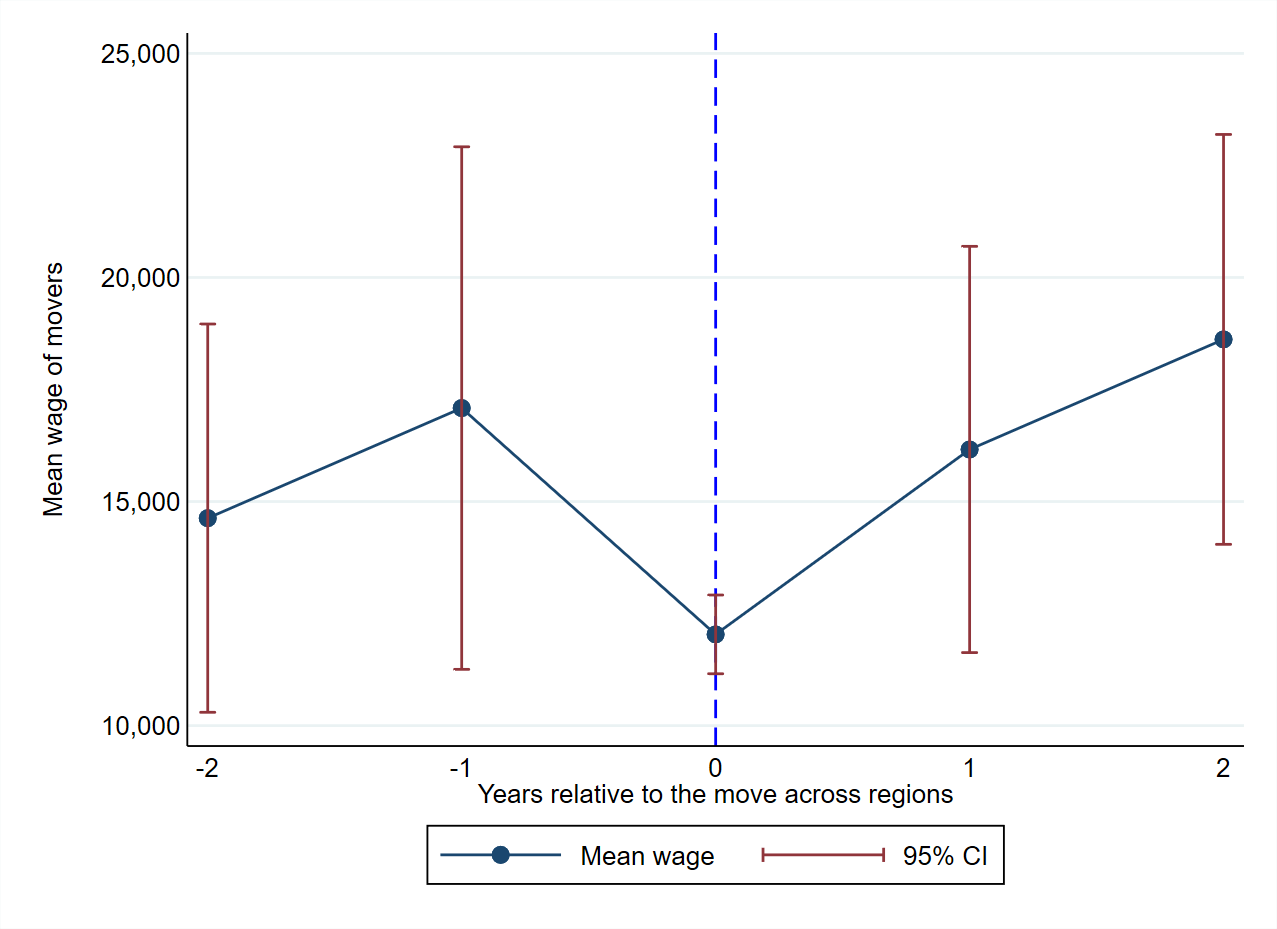
\includegraphics[width = \textwidth]{C:/Users/Zhuxl/Box/projects/ra_code_sample/event_study/output/fig/region_mean_wage.png}
\end{figure}

\begin{figure}[H]
\caption{Average wage of movers between urban and non urban}
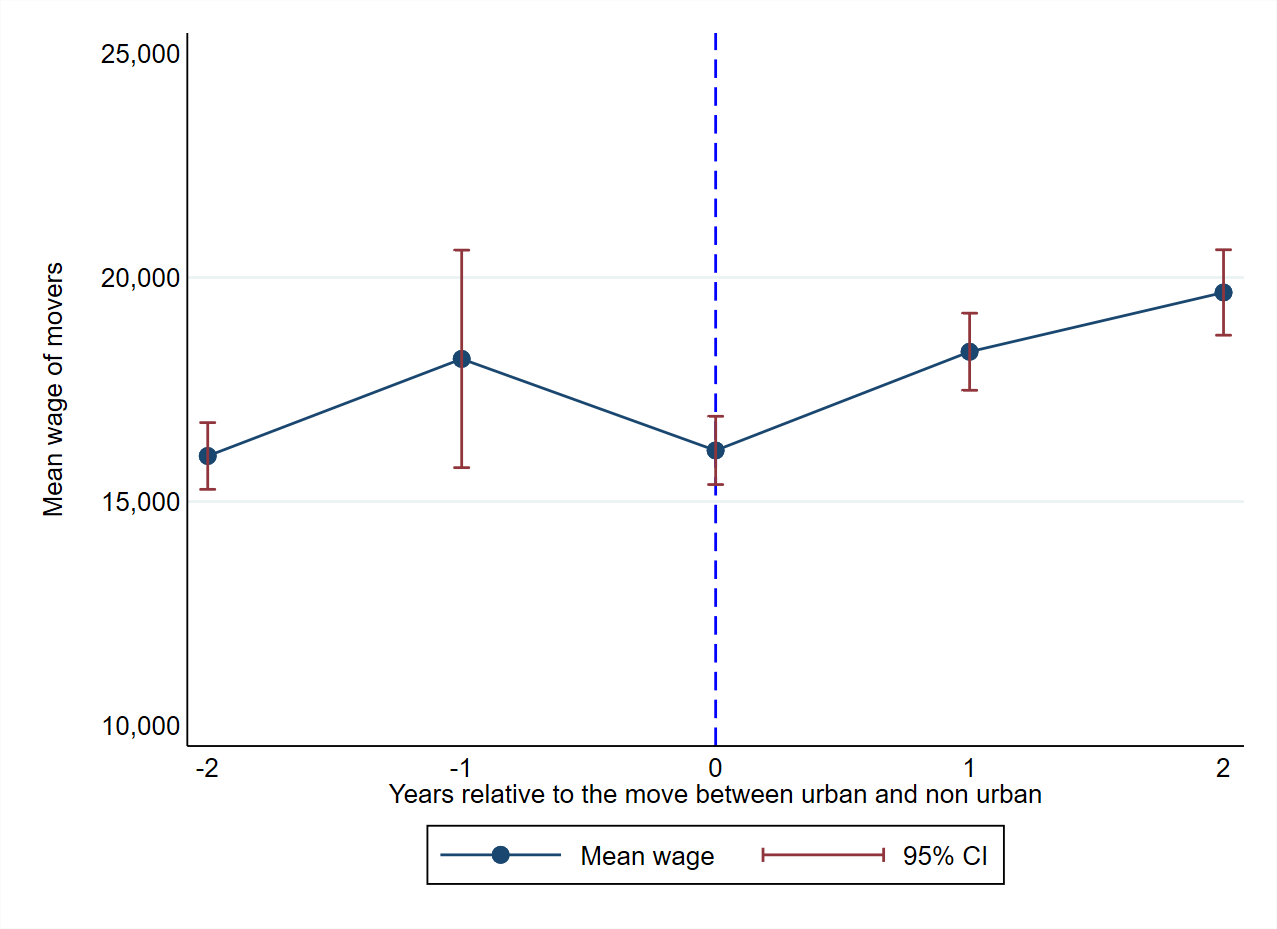
\includegraphics[width = \textwidth]{C:/Users/Zhuxl/Box/projects/ra_code_sample/event_study/output/fig/urban_mean_wage.png}
\end{figure}

\section{Comparing Movers to Stayers} 

Since I had no information on the sampling process of NLSY 79, which was a survey data, I first assumed it is a random sample. Table  4 and 6 reports the differences between the wage of movers and stayers in both region or origin (table 4) and region of arrival (table 6), free of clusters.  Table  5 and 7 reports the differences between the wage of movers and stayers in both region or origin (table 5) and region of arrival (table 7), assuming wage residual was clustered on cohort. 

The model I used for comparison is adapted from the Mincer equation.

To compare movers and stayers in the region of origin:
\begin{equation}
lnw = lnw_0 + \alpha Move from_r  + \beta_1 educ + \beta_2 experience + \beta_3 experience^2 + \beta_4 gender+ \epsilon
\end{equation}

To compare movers and stayers in the region of arrival:
\begin{equation}
lnw = lnw_0 + \alpha Move to_r  + \beta_1 educ + \beta_2 experience + \beta_3 experience^2 + \beta_4 gender + \epsilon
\end{equation}

Where $Move from_r$ is a dummy variable indicating the movers and stayers: $Move from_r = 1$ if the respondent moved out of region $r$, $Move from_r = 0$ if the respondent stayed in the of region $r$. Similarly, $Move to_r = 1$ if the respondent moved into region $r$, $Move to_r = 0$ if the respondent stayed in the of region $r$. 

Age was used as a proxy for experience. 

The rate of return from both moving out of and into region 1 is negative. The rate of return from moving out of region 4 is negative, though the effect was not significant when clustered on cohort. 
\begin{table}[H]
\caption{Compare movers out of a region to stayers at the same region (no cluster of wage residulas)}
{
\def\sym#1{\ifmmode^{#1}\else\(^{#1}\)\fi}
\begin{tabular*}{\textwidth}{@{\hskip\tabcolsep\extracolsep\fill}l*{4}{c}}
\toprule
                    &\multicolumn{1}{c}{Log wage}&\multicolumn{1}{c}{Log wage}&\multicolumn{1}{c}{Log wage}&\multicolumn{1}{c}{Log wage}\\
\midrule
Move from region 1  &      -0.162\sym{***}&                     &                     &                     \\
                    &    (0.0123)         &                     &                     &                     \\
\addlinespace
Move from region 2  &                     &     0.00948         &                     &                     \\
                    &                     &    (0.0119)         &                     &                     \\
\addlinespace
Move from region 3  &                     &                     &     0.00801         &                     \\
                    &                     &                     &   (0.00966)         &                     \\
\addlinespace
Move from region 4  &                     &                     &                     &     -0.0785\sym{***}\\
                    &                     &                     &                     &    (0.0130)         \\
\addlinespace
Age                 &       0.398\sym{***}&       0.361\sym{***}&       0.371\sym{***}&       0.346\sym{***}\\
                    &   (0.00510)         &   (0.00474)         &   (0.00363)         &   (0.00512)         \\
\addlinespace
Age squared         &    -0.00465\sym{***}&    -0.00414\sym{***}&    -0.00432\sym{***}&    -0.00395\sym{***}\\
                    & (0.0000733)         & (0.0000683)         & (0.0000526)         & (0.0000739)         \\
\addlinespace
Education attainment&      0.0402\sym{***}&      0.0471\sym{***}&      0.0501\sym{***}&      0.0344\sym{***}\\
                    &   (0.00295)         &   (0.00281)         &   (0.00208)         &   (0.00287)         \\
\addlinespace
Gender              &      -0.420\sym{***}&      -0.574\sym{***}&      -0.422\sym{***}&      -0.525\sym{***}\\
                    &    (0.0117)         &    (0.0108)         &   (0.00824)         &    (0.0118)         \\
\addlinespace
Constant            &       2.085\sym{***}&       2.668\sym{***}&       2.255\sym{***}&       3.040\sym{***}\\
                    &    (0.0879)         &    (0.0826)         &    (0.0628)         &    (0.0888)         \\
\midrule
Observations        &       33452         &       42146         &       67319         &       34674         \\
\bottomrule
\multicolumn{5}{l}{\footnotesize Standard errors in parentheses}\\
\multicolumn{5}{l}{\footnotesize \sym{*} \(p<0.05\), \sym{**} \(p<0.01\), \sym{***} \(p<0.001\)}\\
\end{tabular*}
}

\end{table}

\begin{table}[H]
\caption{Compare movers out of a region to stayers at the same region (cluster wage residuals on cohort)}
{
\def\sym#1{\ifmmode^{#1}\else\(^{#1}\)\fi}
\begin{tabular*}{\textwidth}{@{\hskip\tabcolsep\extracolsep\fill}l*{4}{c}}
\toprule
                    &\multicolumn{1}{c}{Log wage}&\multicolumn{1}{c}{Log wage}&\multicolumn{1}{c}{Log wage}&\multicolumn{1}{c}{Log wage}\\
\midrule
Move from region 1  &      -0.162\sym{***}&                     &                     &                     \\
                    &    (0.0212)         &                     &                     &                     \\
\addlinespace
Move from region 2  &                     &     0.00948         &                     &                     \\
                    &                     &    (0.0290)         &                     &                     \\
\addlinespace
Move from region 3  &                     &                     &     0.00801         &                     \\
                    &                     &                     &    (0.0157)         &                     \\
\addlinespace
Move from region 4  &                     &                     &                     &     -0.0785         \\
                    &                     &                     &                     &    (0.0343)         \\
\addlinespace
Age                 &       0.398\sym{***}&       0.361\sym{***}&       0.371\sym{***}&       0.346\sym{***}\\
                    &    (0.0255)         &    (0.0299)         &    (0.0223)         &    (0.0232)         \\
\addlinespace
Age squared         &    -0.00465\sym{***}&    -0.00414\sym{***}&    -0.00432\sym{***}&    -0.00395\sym{***}\\
                    &  (0.000404)         &  (0.000440)         &  (0.000332)         &  (0.000362)         \\
\addlinespace
Education attainment&      0.0402         &      0.0471         &      0.0501         &      0.0344         \\
                    &    (0.0246)         &    (0.0218)         &    (0.0215)         &    (0.0192)         \\
\addlinespace
Gender              &      -0.420\sym{***}&      -0.574\sym{***}&      -0.422\sym{***}&      -0.525\sym{***}\\
                    &    (0.0436)         &    (0.0566)         &    (0.0186)         &    (0.0315)         \\
\addlinespace
Constant            &       2.085\sym{***}&       2.668\sym{***}&       2.255\sym{***}&       3.040\sym{***}\\
                    &     (0.383)         &     (0.488)         &     (0.317)         &     (0.296)         \\
\midrule
Observations        &       33452         &       42146         &       67319         &       34674         \\
\bottomrule
\multicolumn{5}{l}{\footnotesize Standard errors in parentheses}\\
\multicolumn{5}{l}{\footnotesize \sym{*} \(p<0.05\), \sym{**} \(p<0.01\), \sym{***} \(p<0.001\)}\\
\end{tabular*}
}

\end{table}

\begin{table}[H]
\caption{Compare movers into a region to stayers at the same region (no cluster of wage residuals}
{
\def\sym#1{\ifmmode^{#1}\else\(^{#1}\)\fi}
\begin{tabular*}{\textwidth}{@{\hskip\tabcolsep\extracolsep\fill}l*{4}{c}}
\toprule
                    &\multicolumn{1}{c}{Log wage}&\multicolumn{1}{c}{Log wage}&\multicolumn{1}{c}{Log wage}&\multicolumn{1}{c}{Log wage}\\
\midrule
Move to region 1    &      -0.201\sym{***}&                     &                     &                     \\
                    &    (0.0134)         &                     &                     &                     \\
\addlinespace
Move to region 2    &                     &     -0.0194         &                     &                     \\
                    &                     &    (0.0127)         &                     &                     \\
\addlinespace
Move to region 3    &                     &                     &      0.0142         &                     \\
                    &                     &                     &   (0.00914)         &                     \\
\addlinespace
Move to region 4    &                     &                     &                     &     -0.0223         \\
                    &                     &                     &                     &    (0.0124)         \\
\addlinespace
Age                 &       0.404\sym{***}&       0.361\sym{***}&       0.369\sym{***}&       0.347\sym{***}\\
                    &   (0.00536)         &   (0.00482)         &   (0.00355)         &   (0.00502)         \\
\addlinespace
Age squared         &    -0.00473\sym{***}&    -0.00413\sym{***}&    -0.00430\sym{***}&    -0.00396\sym{***}\\
                    & (0.0000771)         & (0.0000695)         & (0.0000514)         & (0.0000724)         \\
\addlinespace
Education attainment&      0.0378\sym{***}&      0.0456\sym{***}&      0.0490\sym{***}&      0.0397\sym{***}\\
                    &   (0.00310)         &   (0.00286)         &   (0.00204)         &   (0.00280)         \\
\addlinespace
Gender              &      -0.408\sym{***}&      -0.574\sym{***}&      -0.426\sym{***}&      -0.533\sym{***}\\
                    &    (0.0123)         &    (0.0110)         &   (0.00807)         &    (0.0115)         \\
\addlinespace
Constant            &       1.992\sym{***}&       2.671\sym{***}&       2.319\sym{***}&       2.982\sym{***}\\
                    &    (0.0923)         &    (0.0844)         &    (0.0614)         &    (0.0869)         \\
\midrule
Observations        &       31486         &       39860         &       69861         &       36389         \\
\bottomrule
\multicolumn{5}{l}{\footnotesize Standard errors in parentheses}\\
\multicolumn{5}{l}{\footnotesize \sym{*} \(p<0.05\), \sym{**} \(p<0.01\), \sym{***} \(p<0.001\)}\\
\end{tabular*}
}

\end{table}

\begin{table}[H]
\caption{Compare movers into a region to stayers at the same region (cluster wage residuals on cohort)}
{
\def\sym#1{\ifmmode^{#1}\else\(^{#1}\)\fi}
\begin{tabular*}{\textwidth}{@{\hskip\tabcolsep\extracolsep\fill}l*{4}{c}}
\toprule
                    &\multicolumn{1}{c}{Log wage}&\multicolumn{1}{c}{Log wage}&\multicolumn{1}{c}{Log wage}&\multicolumn{1}{c}{Log wage}\\
\midrule
Move to region 1    &      -0.201\sym{***}&                     &                     &                     \\
                    &    (0.0286)         &                     &                     &                     \\
\addlinespace
Move to region 2    &                     &     -0.0194         &                     &                     \\
                    &                     &    (0.0202)         &                     &                     \\
\addlinespace
Move to region 3    &                     &                     &      0.0142         &                     \\
                    &                     &                     &    (0.0131)         &                     \\
\addlinespace
Move to region 4    &                     &                     &                     &     -0.0223         \\
                    &                     &                     &                     &    (0.0362)         \\
\addlinespace
Age                 &       0.404\sym{***}&       0.361\sym{***}&       0.369\sym{***}&       0.347\sym{***}\\
                    &    (0.0245)         &    (0.0289)         &    (0.0236)         &    (0.0227)         \\
\addlinespace
Age squared         &    -0.00473\sym{***}&    -0.00413\sym{***}&    -0.00430\sym{***}&    -0.00396\sym{***}\\
                    &  (0.000390)         &  (0.000428)         &  (0.000350)         &  (0.000355)         \\
\addlinespace
Education attainment&      0.0378         &      0.0456         &      0.0490         &      0.0397         \\
                    &    (0.0266)         &    (0.0223)         &    (0.0217)         &    (0.0181)         \\
\addlinespace
Gender              &      -0.408\sym{***}&      -0.574\sym{***}&      -0.426\sym{***}&      -0.533\sym{***}\\
                    &    (0.0529)         &    (0.0572)         &    (0.0147)         &    (0.0297)         \\
\addlinespace
Constant            &       1.992\sym{**} &       2.671\sym{***}&       2.319\sym{***}&       2.982\sym{***}\\
                    &     (0.397)         &     (0.493)         &     (0.337)         &     (0.268)         \\
\midrule
Observations        &       31486         &       39860         &       69861         &       36389         \\
\bottomrule
\multicolumn{5}{l}{\footnotesize Standard errors in parentheses}\\
\multicolumn{5}{l}{\footnotesize \sym{*} \(p<0.05\), \sym{**} \(p<0.01\), \sym{***} \(p<0.001\)}\\
\end{tabular*}
}

\end{table}

\end{document}